We will describe the choices we did about representation of the data and communication between modules.

\section{Data model}

First, we describe the data model. All normalized structures of the PPP are JSON-serializable, ie. they are trees made of instances of the following types:
\begin{itemize}
    \item \texttt{Object}
    \item \texttt{List}
    \item \texttt{String}
    \item \texttt{Number}
    \item \texttt{Boolean}
    \item \texttt{Null}
\end{itemize}

We chose to represent all normalized data as trees. To represent sentences, we have 4 kinds of nodes.

\begin{itemize}
    \item \texttt{sentence}: a question in natural language like "Who is George Washington?".
    \item \texttt{resource}: a leaf containing any kind of data (string, integer\ldots).
    \item \texttt{missing}: a leaf which marks missing values.
    \item \texttt{triple}: a 3-ary node:
        \begin{itemize}
            \item \texttt{subject}: what the triple refers to
            \item \texttt{predicate}: denotes the relationship between the subject and the
  object
            \item \texttt{object}: what property of the subject the triple refers to
        \end{itemize}         
\end{itemize}

For example, the work of the NLP is to transform 
\begin{verbatim}
{
    "type": "sentence", 
    "value": "Who is George Washington?"
}
\end{verbatim}
into 
\begin{verbatim}
{
    "type":
        "triple",
    "subject":{
        "type": "resource",
        "value": "George Washington"
    },
    "predicate":{
        "type": "resource",
        "value": "identity"
    },
    "object":{
        "type": "missing"
    }
}
\end{verbatim}

This structure has been chosen for its good adaptability. For instance, we can add other kind of nodes such as intersection, union, node for yes/no questions (triples without missing son), boolean operations etc..

\section{Communication}

Modules communicate with the core via HTTP requests.

The core sends them a JSON object, and they return another one.

The basic idea is that the core iterates requests to modules, which return a simplified tree, until the former gets a complete response.

During these exchanges, we keep a trace of the different steps between the original request and the current tree. The structure of a trace is a list of such trace items:
\begin{verbatim}
{
    "module":
        "<name of the module>", 
    "tree":{
        <answer tree>
    },
    "measures":{
        "relevance": <relevance of the answer>,
        "accuracy": <fiability of the answer>
    }
}
\end{verbatim}

The measure field contains two values: relevance and accuracy.

\begin{itemize}
    \item \texttt{accuracy} is a self-rating of how much the module may have correctly understood (ie. not misinterpreted) the request/question. It's float from 0 to 1.
    \item \texttt{relevance} is a self-rating of how much the tree has been improved (ie. made its way from a question to an useful answer). A positive float (not necessarily greater that 1; another module might use it to provide a much better answer).
\end{itemize}

This form allow each module to access to the previous results, particularly to the user's request. The objects for request and response contains few more information such that the language used.

The data model have been implemented in a nice set of objects in both \href{http://github.com/ProjetPP/PPP-datamodel-Python}{Python} and \href{http://github.com/ProjetPP/PPP-datamodel-PHP}{PHP} in order to help the write of modules.

\begin{figure}
% https://docs.google.com/drawings/d/1toUH24GqwtpvKV7S5gje6GBxfa13R3mxgm8WlAFc_0g/edit?usp=sharing
  \centering
    \label{struct}
    \caption{Architecture of the PPP}
    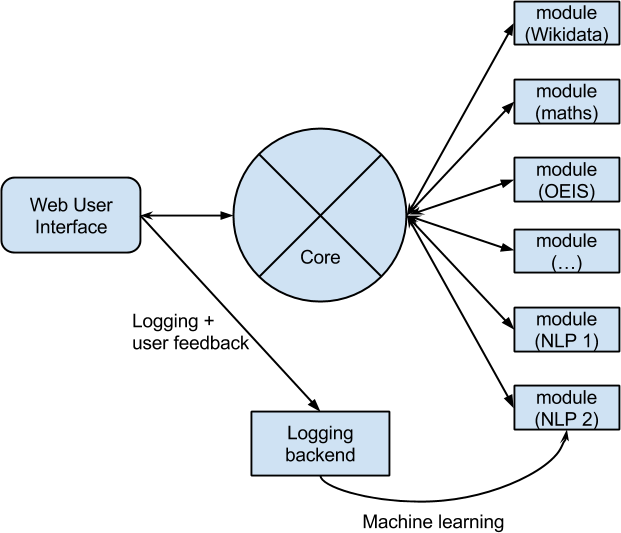
\includegraphics[width=0.5\textwidth]{../ppp_structure.png}
\end{figure}
